\documentclass[11pt,a4paper]{article}

%----------------------------------------------------------------------------------------
%	PACKAGES
%----------------------------------------------------------------------------------------
\usepackage[left=0.8in,top=0.8in,right=0.8in,bottom=0.8in]{geometry} 
\usepackage[utf8]{inputenc}
\usepackage[T1]{fontenc}
\usepackage[default]{sourcesanspro} 
\usepackage{xcolor}      
\usepackage{titlesec}    
\usepackage{enumitem}    
\usepackage{parskip}     
\usepackage{hyperref}
\usepackage{graphicx}

%----------------------------------------------------------------------------------------
%	COLORS & STYLES
%----------------------------------------------------------------------------------------
\definecolor{titleblue}{HTML}{00199e} 
\definecolor{subtitleblue}{HTML}{2ec1e0} 
\definecolor{darktext}{HTML}{222222} 

\color{darktext}
\linespread{0.9} 
\setlength{\parskip}{0.1em} 

\titleformat{\section}{\Large\bfseries\color{titleblue}}{}{0em}{} 
\titlespacing*{\section}{0pt}{0.7em}{0.15em}

\newcommand{\blueitem}[1]{\textcolor{subtitleblue}{\textbf{#1}}}

\setlist[itemize]{label=\textbullet, leftmargin=*, noitemsep, topsep=0pt, parsep=0pt}

%----------------------------------------------------------------------------------------
%	DOCUMENT CONTENT
%----------------------------------------------------------------------------------------
\begin{document}

%--- HEADER ---
%--- HEADER WITH PHOTO ---
%--- HEADER WITH PHOTO ON SAME LINE ---
\noindent
\begin{minipage}[c]{0.73\textwidth}
    {\Huge \textbf{\textcolor{titleblue}{Hamed Razavi Khosroshahi}}}

    \vspace{0.4em}

    Brussels, Belgium \\
    Mobile: +32 472 51 77 10 \\
    Email: h.razavi89@gmail.com \\
    LinkedIn: www.linkedin.com/in/hamed-razavi-khosroshahi/ \\
    GitHub: github.com/HamedRK89 \\
    Scholar: \href{https://scholar.google.com/citations?user=gzbZN8MAAAAJ&hl=en}{Google Scholar Profile} \\
\end{minipage}
\hfill
\begin{minipage}[c]{0.2\textwidth}
    \raggedleft
    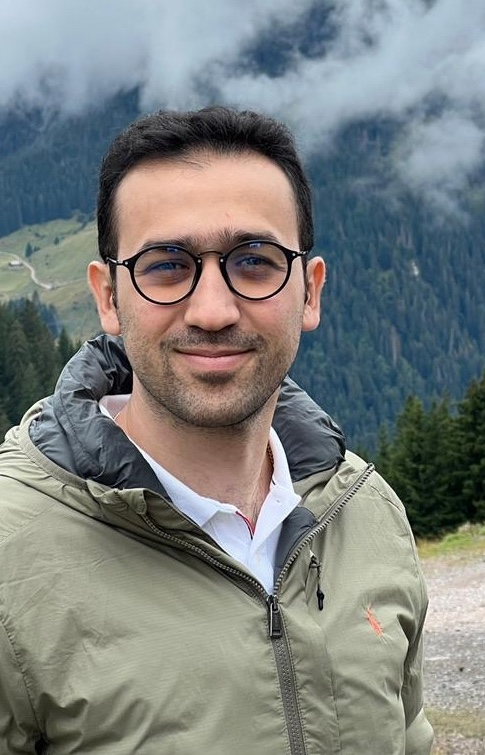
\includegraphics[width=2.5cm]{..\assets\Hamed_.JPG}
\end{minipage}

\vspace{0.6em}

\vspace{0.5em}

%--- PERSONAL PROFILE ---
\section*{Profile}
PhD researcher in computer vision and AI (ULB) specializing in neural rendering, NeRF and 3D reconstruction; experienced in developing and implementing research-grade pipelines in Python and PyTorch and familiar with C++ for engineering integration.

%--- EDUCATION ---
\section*{Education}

\blueitem{Nov. 2021 -- now: Ph.D. Researcher (Expected completion in May 2026)} \\
\textit{Université Libre de Bruxelles, Laboratory of Image Synthesis and Analysis (LISA), Brussels} \\
Full academic scholarship funded by TRAIL/ARIAC\\
\textbf{Supervised by} Prof. Gauthier Lafruit \\
\textbf{Thesis title:} Robust Neural Radiance Fields under Sparse Supervision \\

\vspace{0.3em}
        
\blueitem{Sep. 2012 -- Feb. 2015: M.Sc. Nano-Technology Engineering - Nanoelectronics}\\
\textit{University of Tabriz, Faculty of Electrical and Computer Engineering, Tabriz, Iran} \\
Full academic scholarship\\
\textbf{Supervised by} Prof. Hamed Baghban \\
\textbf{Thesis title:} Design, Simulation, and Fabrication Feasibility of Plasmonic Signal Processor Based on Nanostructures.

\vspace{0.3em}
\blueitem{Sep. 2007 -- Sep. 2011: B.Sc. Electrical Engineering-Electronics} \\
\textit{University of Tabriz, Faculty of Electrical and Computer Engineering, Tabriz, Iran} \\
Full academic scholarship\\
\textbf{Project title:} Design and implementation of a wireless interface for a video transmitter device.

\vspace{1em}

\section*{Research Interests}
\begin{itemize}
    \item Neural Scene Representation and Rendering (NeRF, 3D Gaussian Splatting)
    \item Learning-based 3D Reconstruction
    \item Deep Learning for Medical Image Segmentation
    \item Multimodal and Generative Models
    \item 2D/3D Pose Estimation
\end{itemize}

%--- EXPERIENCE ---
\section*{Professional Experience}
\textbf{PhD Researcher} \hfill ULB \\
        \begin{itemize}
            \item Developed deep learning methods for 3D scene representation and reconstruction (neural rendering / NeRF).
    \item Implemented and evaluated research pipelines in Python and PyTorch; produced scientific reports and papers.
        \end{itemize}

\textbf{Engineer / Research and Development} \hfill Previous company or institute \\
        \begin{itemize}
            \item Designed and developed sensing devices and engineering solutions for precision measurement systems.
    \item Contributed to instrumentation, testing and technical problem solving in R\&D projects.
        \end{itemize}


%--- PUBLICATIONS ---
\section*{Academic Publications}

Available on my \href{https://scholar.google.com/citations?user=gzbZN8MAAAAJ&hl=en}{Google Scholar profile}

%--- PROJECTS ---
\section*{Research Projects}
\textbf{NeRF Research}
\begin{itemize}
\item Worked on neural rendering and sparse-view 3D reconstruction.
\item Investigated robust scene representation methods under limited supervision.
\end{itemize}

%--- SKILLS ---
\section*{Skills}
Computer Vision, Neural Rendering (NeRF), 3D Reconstruction, Deep Learning (PyTorch), Python, C++

%--- REFERENCES ---
\section*{References}

\begin{minipage}[t]{0.48\textwidth}
    \textbf{Prof. Gauthier Lafruit} \\
    Professor at ULB \\
    Laboratory of Image Synthesis and Analysis (LISA) \\
    Université Libre de Bruxelles \\
    Email: gauthier.lafruit@ulb.be
\end{minipage}%
\hfill
\begin{minipage}[t]{0.48\textwidth}
    \textbf{Prof. Mehrdad Teratani} \\
    Professor at Nagoya University \\
    Department of Information and Communication Engineering \\
    Nagoya University \\
    Email: teratani.mehrdad.v5@f.mail.nagoya-u.ac.jp
\end{minipage}

\end{document}